% LaTeX template for Finance summaries
% Stu Alden
%----------------------------------------------------------------------------------------
\author{}

\documentclass{article}

\usepackage{amsmath}
\usepackage{tikz}
\usetikzlibrary{decorations.pathmorphing}

%%%%%%%%%%%%%%%%%%%%%%%%%%%%%%%%%%%%%%%%%%
% Arsclassica Article
% Structure Specification File
%
% This file has been downloaded from:
% http://www.LaTeXTemplates.com
%
% Original author:
% Lorenzo Pantieri (http://www.lorenzopantieri.net) with extensive modifications by:
% Vel (vel@latextemplates.com)
%
% License:
% CC BY-NC-SA 3.0 (http://creativecommons.org/licenses/by-nc-sa/3.0/)
%
%%%%%%%%%%%%%%%%%%%%%%%%%%%%%%%%%%%%%%%%%

%----------------------------------------------------------------------------------------
%	REQUIRED PACKAGES
%----------------------------------------------------------------------------------------

\usepackage[
nochapters, % Turn off chapters since this is an article        
beramono, % Use the Bera Mono font for monospaced text (\texttt)
eulermath,% Use the Euler font for mathematics
pdfspacing, % Makes use of pdftex’ letter spacing capabilities via the microtype package
dottedtoc % Dotted lines leading to the page numbers in the table of contents
]{classicthesis} % The layout is based on the Classic Thesis style

\usepackage{arsclassica} % Modifies the Classic Thesis package

\usepackage[T1]{fontenc} % Use 8-bit encoding that has 256 glyphs

\usepackage[utf8]{inputenc} % Required for including letters with accents

\usepackage{graphicx} % Required for including images
\graphicspath{{Figures/}} % Set the default folder for images

\usepackage{enumitem} % Required for manipulating the whitespace between and within lists

\usepackage{lipsum} % Used for inserting dummy 'Lorem ipsum' text into the template

\usepackage{subfig} % Required for creating figures with multiple parts (subfigures)

\usepackage{amsmath,amssymb,amsthm} % For including math equations, theorems, symbols, etc

\usepackage{varioref} % More descriptive referencing

%----------------------------------------------------------------------------------------
%	THEOREM STYLES
%---------------------------------------------------------------------------------------

\theoremstyle{definition} % Define theorem styles here based on the definition style (used for definitions and examples)
\newtheorem{definition}{Definition}

\theoremstyle{plain} % Define theorem styles here based on the plain style (used for theorems, lemmas, propositions)
\newtheorem{theorem}{Theorem}

\theoremstyle{remark} % Define theorem styles here based on the remark style (used for remarks and notes)

%----------------------------------------------------------------------------------------
%	HYPERLINKS
%---------------------------------------------------------------------------------------

\hypersetup{
%draft, % Uncomment to remove all links (useful for printing in black and white)
colorlinks=true, breaklinks=true, bookmarks=true,bookmarksnumbered,
urlcolor=webbrown, linkcolor=RoyalBlue, citecolor=webgreen, % Link colors
pdftitle={}, % PDF title
pdfauthor={\textcopyright}, % PDF Author
pdfsubject={}, % PDF Subject
pdfkeywords={}, % PDF Keywords
pdfcreator={pdfLaTeX}, % PDF Creator
pdfproducer={LaTeX with hyperref and ClassicThesis} % PDF producer
} % Include the structure.tex file which specified the document structure and layout

\title{\normalfont\ 1-A-1 Simple Interest} % The article title
\date{}  % Suppress date
\pagenumbering{gobble}

\begin{document}

    \maketitle % Print the title/author/date block

    \begin{flushleft}
        Simple Interest is just linear growth in the amount of money.  The simple interest rate is just the rate of growth over each period.
    \end{flushleft}

    \begin{description}
        \item\textbf{A} - amount at the beginning, or principal
        \item\textbf{S} - amount at the end, or final amount
        \item\textbf{i} - interest rate per period expressed as a decimal {(\%/100)}
        \item\textbf{n} - number of periods
    \end{description}

%    To complement this: sometimes you really wish to break a line but LaTeX doesn't
% allow it because you are in vertical mode. In such cases \leavevmode directly
% before \newline or \\ helps. Some people use a quick fix and insert some empty
% space like in ~\\ to repair that.

    \begin{flushleft}
        Then we have
    \end{flushleft}

    \begin{align*}
        Amount \: of \: Interest & = I \\
        & = A \cdot i \cdot n
    \end{align*}

    \begin{flushleft}
        and
    \end{flushleft}

    \begin{align*}
        S & = A + I \\
        & = A(1 + in)
    \end{align*} \\

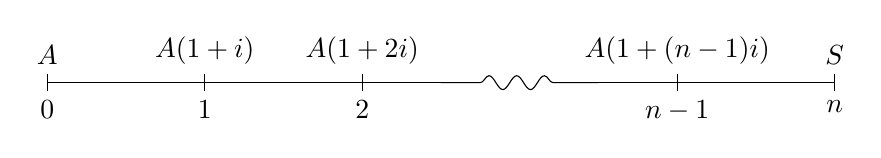
\begin{tikzpicture}
%draw horizontal line with squiggle in middle
    \draw (0,0) -- (5,0);
    \draw[decorate,decoration={snake,pre length=5mm, post length=5mm}] (5,0) -- (7,0);
    \draw (7,0) -- (10,0);

%draw vertical lines
    \foreach \x in {0,2,4,8,10}
    \draw (\x cm,3pt) -- (\x cm,-3pt);

%    {\tiny Text of first line}
%draw nodes
    \draw (0,0) node[below=3pt] {$ 0 $} node[above=3pt] {$ A $};
    \draw (2,0) node[below=3pt] {$ 1 $} node[above=3pt] {$ A(1+i) $};
    \draw (4,0) node[below=3pt] {$ 2 $} node[above=3pt] {$ A(1+2i) $};
    \draw (6,0) node[below=3pt] {$  $} node[above=3pt] {$  $};
    \draw (8,0) node[below=3pt] {$ n - 1 $} node[above=3pt] {$ A(1+(n-1)i) $};
    \draw (10,0) node[below=3pt] {$ n $} node[above=3pt] {$ S $};

    \newline
    \newline

\end{tikzpicture}

\begin{flushleft}
        \textbf{Notes:} \\
    \end{flushleft}


    \begin{itemize}
        \item i is a percentage of the \underline{beginning} amount, but it is credited at the \underline{end} of each period.
        \item Interest rates are annual and the period is a year unless otherwise stated
    \end{itemize}

\end{document}
